\setcounter{reaction}{0}%


\chapter{Background and Related Works} \label{chapter2}

This chapter presents the underlying concepts discussed in this thesis. In the first step, the concept of a digital platform is defined which a theoretical framework for the current project. In the second step, the attention focuses on the research literature about so call Governments as a Platform (GaaP) concept which has direct relevance with the project. Lastly, a quick overview of TOGAF framework is given as it is used for the presentation of the final results.

\section{Digital Platforms}
The concept of a digital platform is a complicated research subject not only because of its omnipresence in today's industries, but also because its multidisciplinary nature \citep{deReuver:2018}. Initially, the concept of a platform was not necessarily binded with digital innovation and digital platforms. The focus was mainly on the economic and business side of the process. 

Classical definition of a platform: A platform was defined as a stable core and a variable periphery <Baldwin and Woodard, 2009> which was primarily realized through modularisation <Henderson and Clark, 1990; Baldwin and Clark, 2000>. The concepts of two-sided markets, network effects, multi-sided platforms, etc. became the top importance.

/Designing digital platform/ 

There is still not much literature about the design principles of DP.

Table with the components of DP

\section{Government as a Platform}



\section{DP for crisis management}
Mention the article about the intention of digitalizing migration process & see artcles of Michailina

\section{TOGAF}
TOGAF is an architecture framework – The Open Group Architecture Framework. TOGAF provides the methods and tools for assisting in the acceptance, production, use, and maintenance of an enterprise architecture. It is based on an iterative process model supported by best practices and a re-usable set of existing architecture assets. (https://www.visual-paradigm.com/guide/enterprise-architecture/step-by-step-enterprise-architecture-tutorial-with-togaf-adm/)

The TOGAF Architecture Development Method (ADM) provides a tested and repeatable process for developing architectures. Each phase of ADM below contains iterative (Continuous) sequence of steps to develop an enterprise-wide Architecture and the possible iterations:
\begin{figure*}[tbp]
\centering
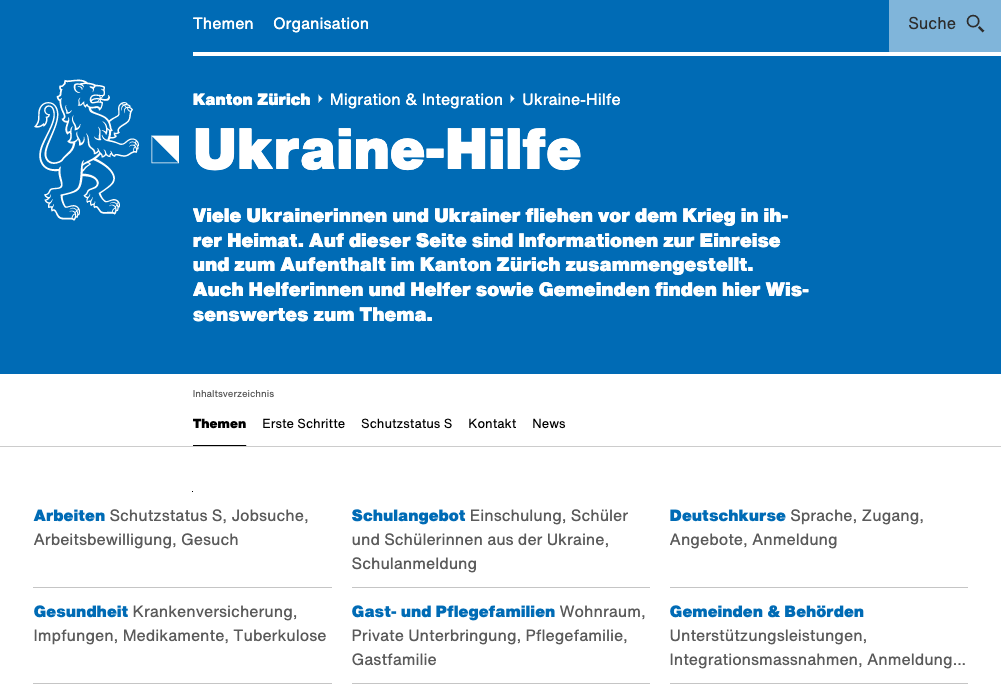
\includegraphics[width=8cm]{Figures/Ukraine_Hilfe.jpg}
\caption{Website of the Canton of Zurich.}
\label{fig:1}
\end{figure*}

This is the classical 

%понять, что делет сам ТОГАФ, какие шаги, какие основные части. Ввести понятия и терминологию

